%TEX root = ../dissertation.tex

\chapter{Background}
\label{chapter:background}
% Context-aware applications
% proximity-based apps
% Technologies
Before describing the solution we need to get a good insight about concepts, technologies available and related work.
Proximity-based applications are a particular kind of context-aware applications.
An application is context-aware when it takes into account the context such as, location, device's orientation, temperature, etc.
Based on this definition, proximity-based applications are context-aware applications that take into account the user's location.
They engage the user while they are on proximity of a given tag.
A tag is a mark with meaning to a given application.
Someone installs tags in a given space.
Then, users can interact with those tags when they are nearby them.
From the given definition of proximity-based application, the concept of Smart Place arises.

Our solution is based on the concept of Smart Place, which we define, in further detail, below, in section \ref{sec:background_smart_places}.
We are going to look at a taxonomy, described in section \ref{sec:background_location}, that allows us to classify the multiple kinds of location to justify our decisions in terms of solution and implementation.
Then, we explore some technologies that could be used in our solution, in section \ref{sec:background_technologies}.
In section \ref{sec:background_related_work} we describe related work providing motivation for the development of our Smart Places solution.
Section \ref{sec:background_summary} summarizes the most important ideas in this chapter.

\section{Smart Places}
\label{sec:background_smart_places}
% Popularity of proximity-based...
% Based on proximity-based
% Explain owners and users
% Figure
% Owner puts tags...
% Relate with location characteristics
A Smart Place is a physical place with tags, which users can interact with using a mobile device such as, a smartphone.
A place's owner installs tags and those tags offer some service to the users when they are nearby.
For instance, a store owner could use these tags to advertise a promotion when the customers are nearby the store.
However, Smart Places are not just for stores.
This concept can be used to any kind of service that benefits from knowing the users to be nearby tags.
For instance, it is possible to build a Smart Restaurant where tags have the information about the table's number and the customers are allowed to call a waiter using their mobile devices, without requiring to type the table's number.

Multiple kinds of people are involved in Smart Places.
There are owners, developers and end users.
Figure~\ref{fig:smart_places_overview} shows how these three kinds of users interact with a Smart Place.
Owners are responsible for managing and installing tags in their places where they want to offer a proximity-based service.
Also, developers are needed to develop these services, for instance, the Smart Restaurant or the store promotions.
Finally, the end users that interact with tags that are installed in Smart Places, using their mobile devices.

\begin{figure}[!ht]
  \centering
    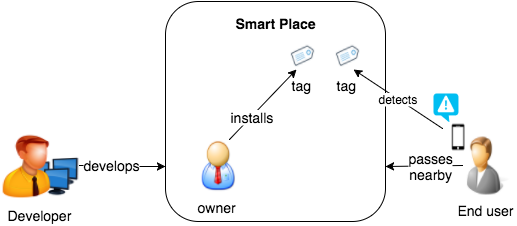
\includegraphics[width=0.8\textwidth, keepaspectratio]{images/smart_places_overview}
    \caption[Smart Places Overview]{Smart Places Overview}
    \label{fig:smart_places_overview}
\end{figure}

\section{Location}
\label{sec:background_location}
% Techniques
% Physical vs symbolic
% Absolute vs Relative
% Computed
% Scale
% Recognition
% Cost
% Limitations
In order to better define what a Smart Place is, we need to have a good insight about concepts related to location.
We have used a taxonomy\cite{location} to classify some properties about location which will allow us to have a better understanding about the concept of Smart Place, in section \ref{sec:background_smart_places}.
Also, these properties are needed to be able to classify the technologies, described in section \ref{sec:background_technologies} and justify if they can be used in the implementation of the concept of a Smart Place.
Using the taxonomy previously mentioned, it is possible to classify location systems in terms of techniques, physical position or symbolic location, absolute or relative position, location computation, scale, cost and limitations.

\subsection{Techniques}
\label{sub:background_techniques}
There are three techniques that can be used to get the device's location.
These techniques are used to compute the location.
A device can use one or combine two or all the three.
The techniques are the following:
\begin{description}
  \item[Triangulation] It can be done via lateration or angulation. Lateration uses distance measurements between three well known points.
  Angulation uses measurements of angles relative to known points;
  \item[Proximity] It takes into account the proximity of the user to a given point
  \item[Scene analysis] It consists in examining a view from a given point.
\end{description}

\subsection{Physical or Symbolic Position}
\label{sub:background_physical_or_symbolic_position}
The device's position can be classified in one of the two types:
\begin{description}
  \item[Physical position] This kind of position refers to a set of coordinates that identifies, unequivocally, a place on Earth where the device is. From this set of coordinates we know exactly where the object is;
  \item[Symbolic location] Unlike physical location, using this kind of positioning it is not possible to identify where the object is. Symbolic can be, for instance, the object is in the kitchen.
  The meaning of its position depends on the application.
\end{description}

One location system can only be classified in one of the two kinds of positioning.
However, physical position can be augmented to also have symbolic information.
For instance, we can have a system that stores coordinates and for each set of coordinates we store symbolic information.
A place on Earth could have symbolic information associated.

\subsection{Computation}
\label{sub:background_computation}
We have multiple ways of obtaining data about location and multiple kinds of location.
However, this data needs to be computed in order to get meaningful information about the object we want to locate.
This computation can be done in one of the two ways:
\begin{description}
  \item[Located object computes its own location] which means that the located object computes its location;
  \item[Location is computed by external infrastructure] meaning that the located object delegates its location computation to an external infrastructure, for instance, a central server.
\end{description}

For instance, \gls{GPS} receivers compute their own location based on signals that come from satellites.
In location systems based on tags, the location's computation is delegated to another machine.

\subsection{Scale}
\label{sub:background_scale}
The scale of a location system refers to the number of objects that is possible to locate using a certain amount of infrastructure or over a given period of time.
For instance, in systems that rely on a fixed number of sattelites, it is possible to serve an unlimited number of receivers.
In systems based on tags, a reader can read a limited number of tags.
In this case, adding more tags can compromise the performance of the entire system.

%\subsection{Recognition}
%\label{sub:background_recognition}
%Recognition refers to the hability, of a location system to recognize individual receivers.
%Location systems based on tags usually have means of recognizing receivers.
%If we assign an \gls{ID} to each receiver each time the receiver reads a tag, that information can be stored and it is possible to know which receiver communicated with that tag.
%There are systems without this capability.
%For instance, \gls{GPS} is a system that is not able to recognize receivers as the satelites do not have any means to recognize receivers.

\subsection{Cost}
\label{sub:background_cost}
There are costs associated to any location system.
It is possible to look at costs in three perspectives:
\begin{description}
  \item[Time costs] Any location system needs time to be spent in installation, administration and other tasks related with its maintenance;
  \item[Space costs] There is always infrastructure associated with any location system. This infrastructure needs space. For instance, if servers are needed, we need to install them in a room;
  \item[Capital costs] The processes and infrastructure associated to a location system requires capital.
  Each mobile unit or infrastructure element has its price. Also, there is people involved. Their salaries are also a capital cost that needs to be taken into consideration.
\end{description}

When comparing multiple location systems, the costs can be a decisive factor. We need not only to take into account the technology characteristics but also the costs.

\section{Location Detection}
\label{sec:background_technologies}
% Possible technologies
% GPS
% QR Codes
% NFC
% Google maps indoor
% BLE
Somehow, the mobile device needs to be able to detect the presence of tags that belong to a given Smart Place.
Multiple technologies can be used.
Some of them require the user interaction, such as the described in section \ref{sub:background_qr_codes}.
Others require the devices to be equipped with extra hardware, such as the one in section \ref{sub:background_near_field _communication}.
We are going to look at these technologies and see which one best fits our purpose, using the taxonomy already introduced.

\subsection{\glstext{GPS}}
\label{sub:background_gps}
% What is it
% How it works
\glsfirst{GPS}\cite{gps} is a location system that uses 24 sattelites plus 3 backups.
Receivers send signals and sattelites answer back. Measurements are taken from this signals in order to receivers be able to calculate their own location.
An object, that we want to locate, only needs a \gls{GPS} receiver in order to to determine its location using this technology.

% Classification
\gls{GPS} uses triangulation as the technique to get the location.
It computes physical location, that is, when an object is located we can look at a map and see where it is.
The located objects have means to compute their own location based on measurements from the satellites' signals.
It is a scalable system because the same number of satelites can handle an unlimited number of \gls{GPS} receivers.
The satelites are not able to recognize individual receivers.
In this system, the major cost is in launching and maintaining the satellites
It cost 12 billion dollars to put them in orbit. The annual operating cost is 750 million dollars\footnote{Source: http://nation.time.com/2012/05/21/how-much-does-gps-cost at 24, December, 2015}.
One limitation of \gls{GPS} is that, it does not work well indoors because the satellite's signal can be weak.

% Requirements
% Advantages and disadvantages
Objects to be located using \gls{GPS} only require an adequate receiver. Most of the mobile devices nowadays are already equipped with these receivers.
This can be a big advantage because it is a low cost solution for users.
However, it is not adequate to locate objects indoors.

\subsection{QR Codes}
\label{sub:background_qr_codes}
% What is it
% How it works
\gls{QR} codes is a type of two dimensional barcode.
The user just needs a camera and software that read these codes.
There are \gls{QR} readers available,
such as, QR Droid\footnote{http://play.google.com/store/apps/details?id=la.droid.qr} for Android, QR Reader\footnote{http://itunes.apple.com/pt/app/qr-reader-for-iphone/id368494609?mt=8} for iOS and QR Code Reader\footnote{http://www.microsoft.com/en-us/store/apps/qr-code-reader/9wzdncrfj1s9} for Windows Phone.
Whenever the user sees one of these codes, he/she can open the \gls{QR} code reader app, scan the code and see the content provided by it.
The content can be an \gls{URL}.
Figure~\ref{fig:qr_code} shows an example of a \gls{QR} code.

\begin{figure}[!ht]
  \centering
    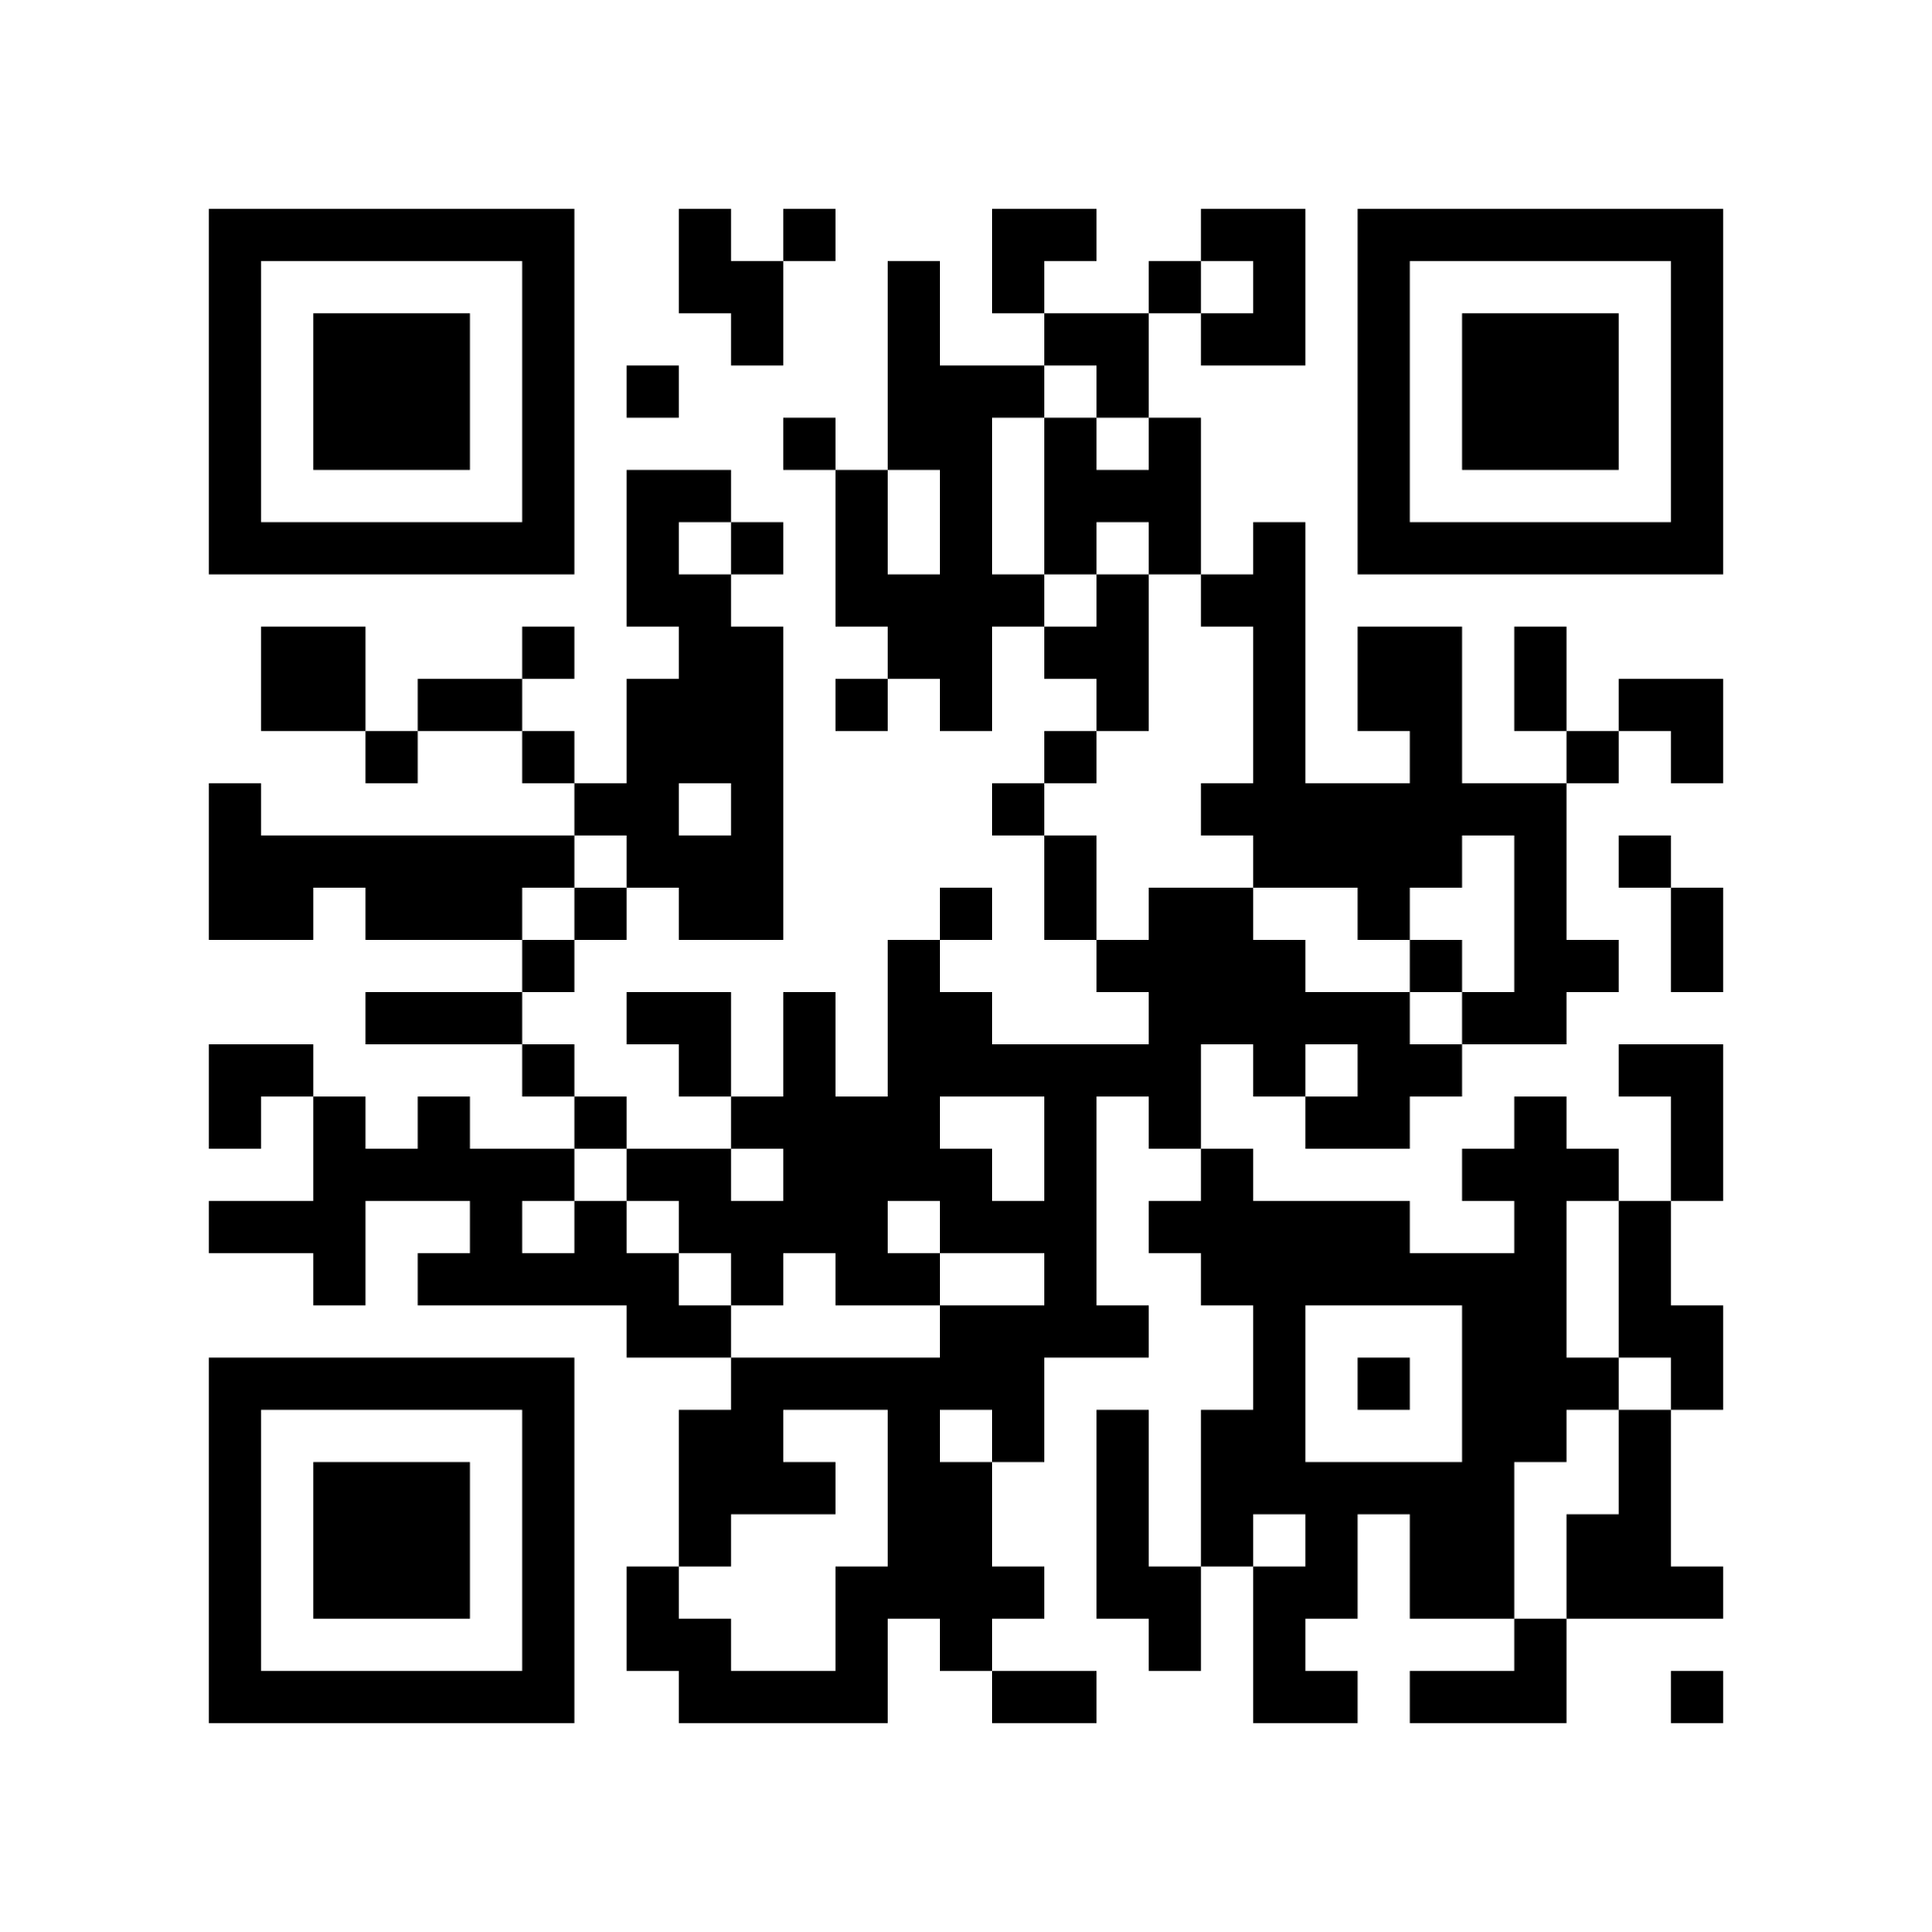
\includegraphics[width=0.3\textwidth, keepaspectratio]{images/qr_code}
    \caption{Example of a QR Code}
    \label{fig:qr_code}
\end{figure}

% Requirements
% Advantages and disadvantages
There is no extra hardware involved.
However, one big disadvantage of this technology is the fact that it requires user interaction.
The user needs to be aware of this kind of codes and also needs to see them wherever they are.
Providing proximity-based services using \gls{QR} codes would be simply using the codes as tags and an app for users to scan these codes and have access to the particular service, that is, Smart Place.

% Related work
There are several applications that use this technology to to get the user's indoor location, such as, the one described in \cite{qr_indoor}.
It uses \gls{QR} codes in combination with \tm{Google} Maps \gls{API}\footnote{http://developers.google.com/maps}.
Others, try to use it to solve real world problems such as hospital overcrowding.
In the work presented in \cite{qr_hospital}, the authors try to use \gls{QR} Codes to identify patients in an hospital.
This information is used in a mobile application that the hospital's staff use to register activities related to the patient.

\subsection{NFC}
\label{sub:background_near_field _communication}
% What is it
% How it works
\glsfirst{NFC}\cite{nfc} is a short distance radio communication technology.
Its range is less than 10 cm.
It can work in one of two modes
\begin{description}
  \item[Active] mode. In this mode, both devices generate their own electromagnetic field alternatively to exchange information;
  \item[Passive] mode. Here, one device generates an electromagnetic field and the other device uses that same field for data transmission.
\end{description}

% Requirements
% Advantages and disadvantages
Simillary to \gls{QR} Codes, this technology requires the user interaction and his/her awareness of the existence of these kinds of tags.
Also, devices need to be equipped with \gls{NFC} readers.
% Related work
This technology is already being used for payments, such as \tm{Apple} Pay\footnote{http://www.apple.com/apple-pay/}.

% Get references to this...
\subsection{WiFi Signal Mapping}
\label{sub:background_google_maps_indoor}
% WiFi mapping
\gls{WiFi} can be used as a location detection technology.
\gls{WiFi} fingerprinting\cite{wifi_fingerprinting} uses the \glspl{AP} signal's strength to locate the receiver inside a building.
Google Maps Indoor is an example of an application that uses this technique to locate the user indoors.

% What is it
% How it works
Google Maps allows users to navigate all over the world and gives access to satellite images.
There are mobile apps for Android and iOS.
With more than \num{1e9} installs on Google Play Store and an average rating of 4.3\footnote{Source: http://www.appannie.com/apps/google-play/app/com.google.android.apps.maps in 23 December 2015}, we can say it is a very popular and mainstream app.
When installed on a smartphone, it uses multiple sensors such as, \gls{GPS} and accelerometer, in order to get the user's location.
However, since it relies on \gls{GPS} it does not work well indoors.
Google Maps Indoor\footnote{http://www.google.com/maps/about/partners/indoormaps} is an extension which allows the user to navigate inside a building.
Figure~\ref{fig:google_maps_indoor} shows an example of Google Maps Indoor.

\begin{figure}[!ht]
  \centering
    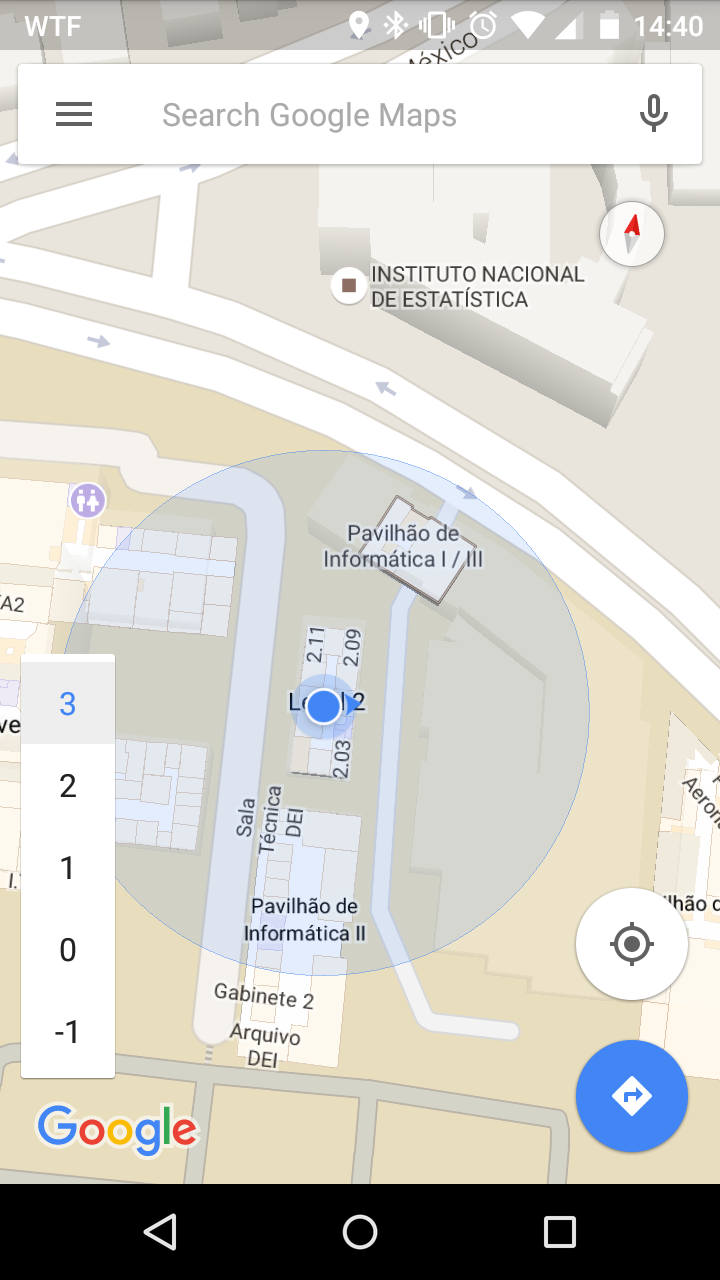
\includegraphics[width=0.3\textwidth, keepaspectratio]{images/screenshots/google_maps_indoor}
    \caption[Google Maps Indoor]{Screenshot of Google Maps with indoor functionality}
    \label{fig:google_maps_indoor}
\end{figure}

% Requirements
% Advantages and disadvantages
This service uses sensors already provided by the mobile device and it does not require extra sensors inside the building.

\subsection{Bluetooth Low Energy}
\label{sub:background_bluetooth_low_energy}
% What is it
% How it works
\glsfirst{BLE}\cite{ble} is a short range wireless communication technology, developed by Bluetooth \gls{SIG}\footnote{http://www.bluetooth.org}.
It is more focused on low power consumption than classic Bluetooth.
To take advantage of this technology the mobile device needs to be equipped with Bluetooth version 4.0\cite{bluetooth_specification} or above.
However, to be able to use it in order to get the user's indoor location, a protocol is needed.
There are two protocols that can be used: iBeacon\footnote{http://developer.apple.com/ibeacon}, developed by \tm{Apple} and Eddystone\footnote{http://github.com/google/eddystone}, developed by \tm{Google}.

% Protocols: ibeacon and eddystone
The iBeacon protocol works with small devices named beacons that broadcast a sequence of bytes, which acts as an identifier allowing to build proximity-based applications\cite{ibeacon_book}.
Figure~\ref{fig:ibeacon_message} shows the structure of this sequence of bytes, where it is possible to see three parts:
\begin{description}
  \item[\gls{UUID}] has 16 bytes (128 bits) and it identifies the organization that the beacon belongs to;
  \item[Major] has two bytes (16 bits) and it identifies a group of beacons that belong to a given organization identified by the \gls{UUID};
  \item[Minor] has two bytes (16 bits) and it identifies each individual beacon in the group identified bu the Major value.
\end{description}
In this protocol, location is reported to an application using one of the two operations:
\begin{description}
  \item[Monitoring] This operation is called when the beacon and the mobile device are in the same space;
  \item[Ranging] It is related to a single beacon. The distance from a mobile device to a beacon is estimated using its transmissions.
\end{description}

\begin{figure}[!ht]
  \centering
    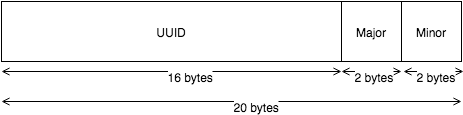
\includegraphics[width=0.6\textwidth, keepaspectratio]{images/ibeacon_message}
    \caption[iBeacon message structure]{Structure of the sequence of bytes transmitted in iBeacon protocol}
    \label{fig:ibeacon_message}
\end{figure}

In Eddystone protocol the beacons also advertise a sequence of bytes.
However, there are three types of messages that beacons can broadcast to mobile devices nearby\footnote{http://github.com/google/eddystone/blob/master/protocol-specification.md}:
\begin{description}
  \item[Eddystone-UID]
  It broadcasts an unique 16 byte (128 bits) identifier. The first 10 bytes are for the namespace, which is used to distinguish groups of beacons and the remaining 6 are for the instance's \gls{ID}, which is used to identify individual beacons inside the same namespace;
  \item[Eddystone-URL]
  As the name suggests, it broadcasts an \gls{URL};
  \item[Eddystone-TLM]
  Here, telemetry information about the beacon is transmitted such as battery voltage and device's temperature.
\end{description}

% Requirements
% Advantages and disadvantages
The main advantage of this technology is that it only requires that the mobile device has Bluetooth 4.0.
However, to develop proximity-based applications, we need to deploy some beacons that use the iBeacon or the Eddystone protocol.
Fortunately, the extra hardware is the space owner's responsability.
The user does not need anything else besides his/her mobile device.

Using this technology, if developers want to map beacons to more kinds of information, only the mentioned protocols are not enough.
We need a backend to store the mapping between the beacons and that information.
Besides developing the application itself, developers also need to deal with the backend and all the concerns around any distributed system, such as, scalability, performance, etc.

\subsection{Comparison}
\label{sub:background_overview}
% Main advantages of each one
% The chosen one (BLE ibeacon)
% Why
There are no perfect location systems. Every system has its own limitations.
There are ones that do not work well indoors, such as the \gls{GPS} because it cannot get the sattelites' signal.
If we want a location system that would work indoors, maybe a tag based system is a better fit.
When choosing a system, this is important because one might not require extra hardware and it leads to a low cost system but, if the limitations compromise its performance it is better to pick one with higher costs.
Multiple technologies were taken into consideration.
Ones are tag based, such as \gls{QR} codes, \gls{NFC} and \gls{BLE} that can be used to provide symbolic location.
Others, such as \gls{GPS} and Google Maps Indoor, are used to provide physical location but can be augmented to provide symbolic location.
However, \gls{GPS} does not work properly indoors and Google Maps Indoor requires that buildings are mapped first. This mapping can be performed by a team from \tm{Google} or by users.
Each technology was classified in terms of techniques, type of location (physical or symbolic), computation, scale and costs.
This classification was made using the taxonomy introduced in section \ref{sec:background_location} and is summarized in Table~\ref{tab:technologies}.

\includeTable{technologies}

% Discussion of technologies
The concept of Smart Place is based on proximity and symbolic location.
Also, it is supposed to work indoors.
% GPS
\gls{GPS} is a location system that uses triangulation to provide physical location.
It is possible to augment physical location in order to provide symbolic.
However, it only works properly where it has a good receiption of the satellites' signal.
Since the concept of Smart Place is a concept connected to an indoor space, the \gls{GPS} is not a good option even if we augment it to provide symbolic location, because it does not work properly indoors.

% QR and NFC
\gls{QR} Codes and \gls{NFC} are based on the proximity technique.
They can provide symbolic location if enough data is stored in an external infrastructure.
The scale is dictated by this infrastructure and not not by the device that is being located.
The costs depend on the amount of infrastructure.
The main limitation of both is that it is only possible to read a tag at a time.
\gls{QR} Codes require that we spread codes which can be shown in a piece of paper.
\gls{NFC} tags are more expensive.
However, both would take us to a solution where the user interaction is required, that is, the user needs to be aware of existing tags and start the interaction instead of just being notified that a given proximity-based service is available at that location.
% Google Maps Indoor
Smart Places could be implemented using Google Maps Indoor.
This technology is based on triangulation technique and provides physical location.
Similar to \gls{GPS} it can be augmented to provide symbolic location requiring a given amount of external structure, which is what scale depends on and the major cost here.
This would lead to a solution where no extra hardware is needed.
However, it requires a previous mapping of the building before users are able to navigate in it using Google Maps Indoor.
% BLE
\gls{BLE} is a good fit for our purpose because, it is based on proximity and can be used to provide symbolic location.
It does not have any costs for the users besides the acquisition of the mobile device.
We can place the beacons wherever we want and where it makes sense for the service we want to provide.
Also, using this technology, the mobile app that will handle the nearby beacons can be running in background.
This way, the user does not to be aware of any tags and he/she can be notified if a proximity-based service is found.

% Final decision -> BLE
The final decision was to pick \gls{BLE} because it has the best tradeoff between cost and kind of location it provides. Using this technology we have symbolic location. With the adequated infrastructure it is possible to associate any kind of information to each tag.
It requires extra hardware but this is the responsability of who manages the place where the tags will be deployed.
The user does not need anything else but a mobile device with Bluetooth, version 4.0 or later.
Three beacons, from \tm{Estimote} were used in the implementation of our solution, described in chapter \ref{chapter:implementation}.

\section{Related Work}
\label{sec:background_related_work}
% Related work...
Here we discuss related work in order to have a good insight about the possibilities and existing solutions for the problem we are trying to solve.

\subsection{Proximity-based Apps}
\label{sub:background_ble_beacons_applications}
% Why
% For each one: What, Pros, Cons
\gls{BLE} Beacons were
used to develop our solution, based on the concept of Smart Places.
Some applications where this technology is used
are presented here to
get good insights about the potential use cases of this
technology and the apps developed using it.
\begin{description}
  \item[BlueSentinel\cite{Conte2014}]
  is a
  occupancy detection system for smart buildings
  that uses \gls{BLE} Beacons to detect the presence of
  people. The concept of a smart building
  is similar to Smart Place
  due to the existence of sensors and actuators.
  It is focused on the power efficiency of the
  building.
  The idea is to optimize energy
  consumption according to people's presence.
  For instance, if there are no people in a given room
  the heating system can be turned off.
  In this solution the users have to install
  an app that will get the beacons' signal and
  send data to a server, which will process it
  and send requests to actuators in order to
  perform actions to optimize the
  building's power efficiency.
  Unfortunately, there is a limitation
  of iBeacon protocol implementation
  in iOS.
  Beacons can be received by the apps
  only when these are active. When the apps are in
  background they are waken up only to handle
  enter/exit region events. To circumvent this
  limitation the authors developed custom
  beacons which advertise more than one region
  in a cyclic sequence. These custom beacons
  were created using an
  Arduino\footnote{http://www.arduino.cc/}
  and a Bluetooth \gls{USB} dongle.
  Since this solution is a native app
  users have to install it in order
  to make the smart building work to
  optimize power efficiency.
  Once the user starts the app, he/she does not
  need to interact with it anymore since it
  will run in background.
  \item[BlueView\cite{Chen2013}]
  is a system to help
  visually impaired people to perceive some points of interest.
  This solution has two main components: The viewer device
  and the \glspl{BP}. The first one is a mobile phone,
  carried by the user, which is bluetooth enabled.
  The \glspl{BP} are just bluetooth tags instead of
  \gls{BLE} Beacons. The name of a point of interest is associated with the
  \gls{MAC} address of the tag which it is associated to.
  The steps involved in using the system are the
  following: first, the viewer device will scan
  for nearby \glspl{BP}; then, a list of the names of
  \glspl{BP} is created. This list is refreshed anytime a new
  \gls{BP} is detected and the user is informed through auditory feedback.
  The second step consists of the user using
  the viewer's device establishing a connection with a \gls{BP}
  attached to an object. Finally, using audio prompt, the \gls{BP}
  will assist the user in locating the object.
  Despite of this solution being a mobile app, installed
  in the viewer's device the authors do not have in
  consideration the typical concerns of any mobile app,
  such as the energy consumption.
  The authors tested the application, in 2013,
  using Nokia N70 as the viewer device.
  This solution could be implemented using \gls{BLE} Beacons
  and the viewer device could be any Android or iOS smartphone.
  \item[ContextCapture\cite{Antila2011}]
  uses context-based information to allow users to
  add more information to their status updates
  in the main social networks, such as
  Facebook\footnote{http://www.facebook.com} and
  Twitter\footnote{http://twitter.com}.
  This work had two main goals: first, demonstrate technical
  aspects of collaborative context such as,
  how to get contextual information from
  surrounding devices and how they can be used
  as a source of contextual information;
  second, test and analyze the user experience of
  context-aware systems.
  The user can decide the abstraction level (coordinates,
  address or semantic label).
  The authors implemented a mobile app and a
  server integrated with Facebook and Twitter.
  Context information comes from the smartphone itself,
  from its sensors and from the nearby devices through
  Bluetooth.
  Devices can be other smartphones or \gls{BLE} Beacons which
  are used for indoor location.
  Similar to \cite{BenAbdesslem2014}, devices communicate
  with each other as a network.
  Using this solution, the user can create status updates
  in the mentioned social networks in the format shown in Listing~\ref{lst:context_capture_status_update}:
  \begin{listing}[H]
      [User-defined message]

      Sent from [Location] while [Activity]

      [Description] [Topic] and [Applications Activity] with
      [Friends].
    \caption[ContextCapture update format]{Format of status updates in ContextCapture}
    \label{lst:context_capture_status_update}
  \end{listing}
\end{description}

\subsection{Context-aware applications}
\label{sub:frameworks_context_aware}
In this section we describe related work about the
development of mobile native and web
context-aware applications.
Since we have created a framework to develop
proximity-based services, the state
of the art of existing frameworks that deliver
context information to the apps will be presented.
\begin{description}
  \item[Frameworks for developing distributed
  location-based applications:]
  There are frameworks to develop location-based
  applications.
  In the work presented in Krevl et al.\cite{Krevl2006},
  a framework
  was developed to allow developers to build
  location-based apps. Location information can come
  from any source, such as \gls{GPS}, Bluetooth and \gls{WiFi} receivers.
  The authors discuss some benefits and limitations
  of several technologies for getting the
  user's location.
  In terms of architecture, the main components
  are:
  \begin{itemize}
  \item
  Devices that are used to get location data, such as
  the ones already mentioned;
  \item The users' mobile devices;
  \item The Database Server, which is where the mapping
  between geographical coordinates and location
  information is stored;
  \item And, the Application Server, which provides web services for
  mobile clients.
  This server also communicates
  with the Database Server.
  \end{itemize}
  The mobile device gets geographical coordinates
  from any source and send that data in a
  \gls{SOAP}\cite{Seely:2001:SCP:560836} message,
  to the appropriate web service in the Application
  Server. This server communicates with the Database Server
  to query the database, which sends back a response with
  location information, if there is any, for that
  particular group of geographical coordinates.
  The authors did not evaluate the system.
  \item[Dynamix\cite{dynamix}]
  is a framework to develop
  mobile native and web apps that allows them to receive
  context information for instance, position and device's
  orientation. This framework has plugins that get
  one or more sensor's raw data and turn that into event
  objects that contain more high-level information.
  This framework supports many kinds of context information
  and it is possible to develop more plugins to allow the
  apps to generate additional events that are not
  already supported.
\end{description}

\subsection{Discussion}
\label{sub:solution_related_work_discussion}
In order to get a good insight about the potential of proximity-based services, we analyzed three applications.
The BlueSentinel is a system that uses \gls{BLE} beacons to detect the presence of people in a building. It tries to optimize energy consumption based on people's presence.
Another one, BlueView, is a system to help visually impaired people to be aware of some points of interest.
The third is the ContextCapture that allows users to create status updates on social networks using context information.

We introduced a framework to develop distributed location-based applications and a more generic one that targets the development of context-aware applications.
For each one, we described the idea, its main components, in order to get an overview about their limitations, which we try to circumvent in our solution.
However, most of them only allow developers write native apps, that is, apps written for a specific platform that will run only on it.
This leads to a situation where the user needs to install one app, in his/her mobile device, for each proximity-based service he/she wants to use.
In order to circumvent this limitation, our Smart Places solution allows developers
to use the same technologies that are used for any web application such as \gls{HTML}, \gls{CSS} and Javascript to build Smart Places allowing them run on a web browser that can be embedded in a mobile app. This way, users only need to install one app to discover and use proximity-based services following the Smart Places approach.

The framework described in Krevl et al.\cite{Krevl2006} offers abstractions for the location information sources.
Geographical coordinates can
come from any source.
It is a good approach for
mobile native apps but it does not support web apps.
The authors do not take into consideration
constraints in terms of resources, such as
Internet connection and battery.
Since most users have limited data plans for
their smartphones and \gls{SOAP} messages can
grow in size due to its \gls{XML} format,
a more efficient message encoding could be used
instead, for instance \gls{REST} using \gls{JSON}.

To achieve our goal, our framework could be just a
plugin for Dynamix. The plugin would
need to get the beacon's raw data and
turn that into a more high-level information
using a backend. In this framework,
the user needs to install an app that manages the service
that runs in background and needs to define some
security policies such as which information the app can have access to or which sensors it can use.
This could mean a big overhead since we are more focused on developing proximity-based applications that do not require such complex security policies because in this kind of applications, there is only need to access the device's sensors that could provide positioning data to the applications

\section{Summary}
\label{sec:background_summary}
% Location
% -> Introduced taxonomy (techniques, physical vs sumbolic, computation, scale, recognition, cost and limitations)

Smart Places are based on the proximity technique and symbolic location.
Also, we need to take into account the cost and limitations because we want a solution as low cost as possible, in terms of time and capital, for end users, owners and developers.

In this chapter we introduced a taxonomy to classify location systems in terms of techniques, physical or symbolic location, computation, scale, cost and limitations.

% Smart Place (based on taxonomy)
The concept of Smart Place was defined as a place with tags, that provides a service to users when they approach those tags.
Using the taxonomy with property definitions we need a location system that is based on the proximity technique and provides symbolic location.

% Technologies
% -> GPS, QR Codes, NFC, GMI, BLE
% -> Chose BLE because...
In our solution, we needed to choose a location technology.
We analyzed \gls{GPS}, \gls{QR} Codes, \gls{NFC}, Google Maps Indoor and \gls{BLE}, according to the taxonomy introduced before.
We concluded that the \gls{BLE} using ibeacon protocol is the best option because it works well indoors, unlike \gls{GPS}.
Also, it does not require user interaction, as it is in \gls{QR} Codes or \gls{NFC}.
Using this technology, owners can place tags anywhere without the need to first map the entire area, as it is needed in Google Maps Indoor.

We explored related work about existing proximity-based applications and tools to develop this kind of applications.
In most solutions users have to install one app for each proximity-based service they want to use. There is not a solution to allow users to discover new services and use them as soon as they found them.
Our solution described in the next chapter tries to solve these limitations and turn the development and usage of services based on Smart Places in easy processes.
